\documentclass[
    a4paper,
    12pt,
    fleqn,
    % twoside
]{report}
\usepackage{duarte}
\usepackage{blindtext}
% ----------------------------
\begin{document}

% ============================
% CAPA
\begin{titlepage}
    
\sffamily
\centering
{\Large\bfseries São Paulo State University}

{\Large School of Engineering of Ilha Solteira}

\vfill

{\LARGE\bfseries Machine Learning: Optimizing Smart Systems with Artificial Intelligence}

\vfill

\begin{tabular}{ll}
    Student:        & Gabriel D. Silva \\
    Professor:      & Douglas D. Bueno
\end{tabular}

\vfill

Research Report --- Iniciação Científica 

\vfill

UNESP \\
Ilha Solteira - SP \\
2023
\end{titlepage}


% \begin{titlepage}
%     \sffamily
%     \begin{center}
%      {\LARGE \bfseries SÃO PAULO STATE UNIVERSITY}
     
%      {\LARGE School of Engineering of Ilha Solteira}
     
%      \vfill
     
%      {\Huge \bfseries DEEP LEARNING: APPLICATIONS IN THE MECHANICAL ENGINEERING CONTEXT}
     
%      \vfill
     
%      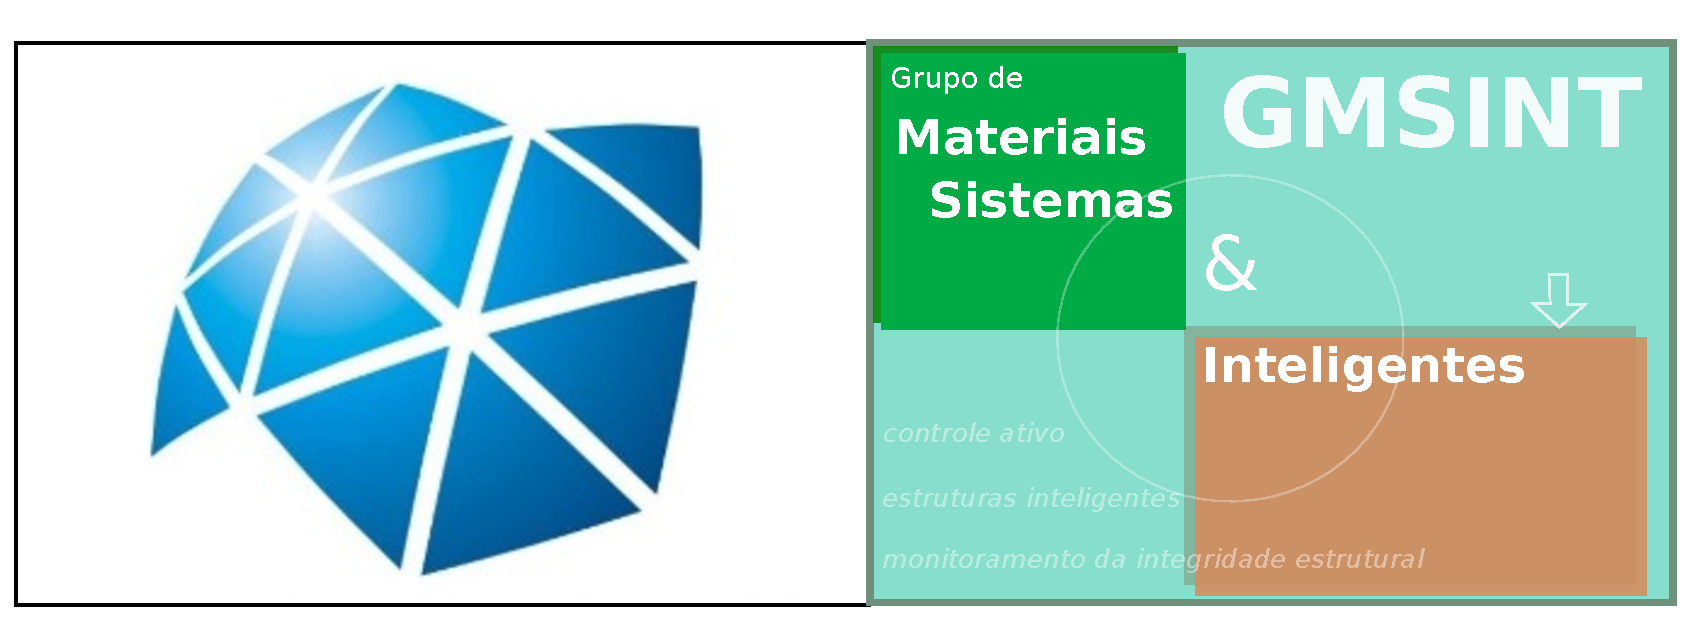
\includegraphics[width=\textwidth]{figures/logos/gmsint_logo.pdf}
     
%      \vfill
     
%      \begin{minipage}{0.7\textwidth}\centering
%       {\large \bfseries Research Report -- Iniciação Científica}
      
%       {\large \bfseries Student: Gabriel D. Silva}
      
%       {\large Professor: Douglas D. Bueno}
      
%      \end{minipage}
     
%      \vfill
     
%      {\large \bfseries UNESP}
     
%      {\large \bfseries Ilha Solteira -- SP}
     
%      {\large \bfseries 2023}
%     \end{center}
%    \end{titlepage}
% ----------------------------

% ============================
% RELATÓRIO DE PESQUISA
\setcounter{page}{1}
\pagenumbering{roman}
\renewcommand{\thepage}{\textit{\roman{page}}}
\pagestyle{empty}
\begin{center}
	\vspace{100pt}
	{\Large\scshape\bfseries Research Report}
\end{center}
\noindent
The present report approaches a way to improve smart systems. Through artificial intelligence applied in the mechanical engineering field, it provides a consistent algorithm that can reads data, trains the machine and provides results about the situation and what to do with it. It will be studied two cases, one of them using machine learning classical techniques to determine the forces applied to a unnamed aerial vehicle and other using deep learning techniques like neural networks in the structural health monitoring area. 

\noindent
\textcolor{red}{Complete after the research is done.}

\noindent
{\bfseries Keywords:} machine learning, structural health monitoring, unnamed aerial vehicle

\clearpage
% ----------------------------

% ============================
% LISTA DE FIGURAS
% {\sffamily\listoffigures}
% \listoffigures
{%
\let\oldnumberline\numberline%
\renewcommand{\numberline}{\figurename~\oldnumberline}%
\listoffigures%
}
\newpage
% ----------------------------

% ============================
% LISTA DE TABELAS
% {\sffamily\listoftables}
% \listoftables
{%
\let\oldnumberline\numberline%
\renewcommand{\numberline}{\tablename~\oldnumberline}%
\listoftables%
}
% \newpage
% ----------------------------

% ============================
% LISTA DE ABREVIAÇÕES
% \setlist[description]{leftmargin=!, labelwidth=5em} % Change for glossaries
\printglossary[title=List of Acronym, nonumberlist]
% \setlist[description]{style=standard} % reset settings back to default
\newpage
% ----------------------------

% ============================
% SUMÁRIO
% {\sffamily\tableofcontents}
\tableofcontents
\newpage
% ----------------------------

% ============================
% FORMATAÇÕES EXTRAS
\setcounter{page}{1}
\pagenumbering{arabic}
\pagestyle{fancy}
% ----------------------------

% ============================
% SEÇÕES
\chapter{Literature Review}\label{sec:literature_review}

This chapter deals with the history, the main concepts and some practical cases of \gls*{shm} inside the industry and academic area, besides showing how it may be used in the railway crack detection context.
Next, in the dynamic field, it will be studied the main mechanical concepts to get the necessary understanding to an \gls*{uav} motion as well the basics to know how an \gls*{uav} can be controlled.
Then, it will be shown the mathematics behind the algorithms of deep learning that will be implemented in the \cref{sec:results}. 
Finally, the way how the algorithms are going to be implemented and the tools necessary to achieve the desired \gls*{nn}.

\chapter{Literature Review}\label{sec:literature_review}

This chapter deals with the history, the main concepts and some practical cases of \gls*{shm} inside the industry and academic area, besides showing how it may be used in the railway crack detection context.
Next, in the dynamic field, it will be studied the main mechanical concepts to get the necessary understanding to an \gls*{uav} motion as well the basics to know how an \gls*{uav} can be controlled.
Then, it will be shown the mathematics behind the algorithms of deep learning that will be implemented in the \cref{sec:results}. 
Finally, the way how the algorithms are going to be implemented and the tools necessary to achieve the desired \gls*{nn}.
\section{Structural Health Monitoring}

\subsection{Definition}

According to  \citet{balageas2010}, the \gls*{shm} main purpose is to provide, during the life of a structure,  a diagnosis of: the state of the constituent material; the different parts of the structure; and the full assembly of each part that makes the structure as a whole. 
It is an improved way to make non-destructive evaluation.
It can be applied in several areas such as civil infrastructure, like bridges and buildings; aerospace, like airplanes and spaceships; and mechanical, like machines.

% \begin{figure}[H]
%     \centering
%     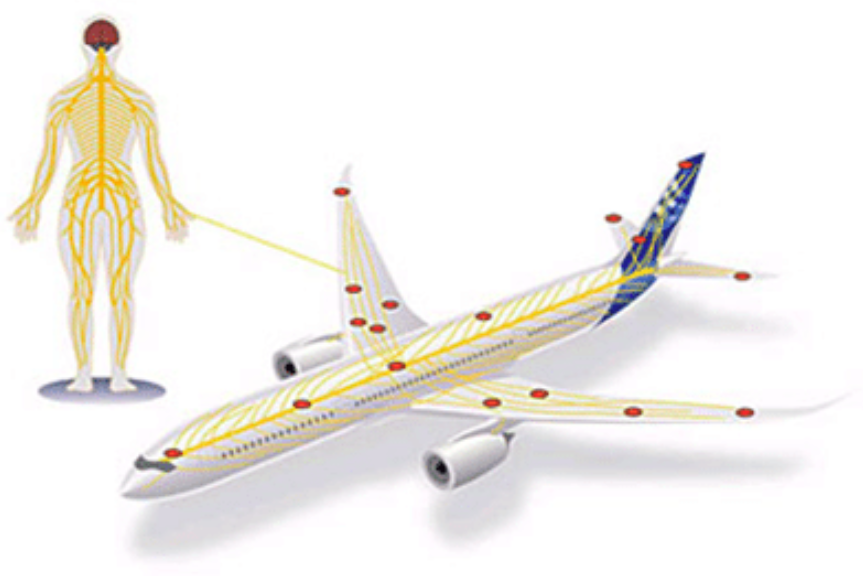
\includegraphics[width=0.6\textwidth]{figures/2methodology/shm/smh_nervous_system.png}
%     \caption[SHM and human nervous system analogy]{\gls*{shm} and human nervous system analogy. Source: \citet{blanckenstein2015}}
%     \label{fig:shm_nervous_system}
% \end{figure}

Furthermore, it also can be associated as an analogy to the human nervous system. Just like the sensors send a signal to the central processor, the human 
senses send a signal to the brain to make the recognition of what is happening.

\subsection{Brief History}

The \gls*{shm} development began back in the 20th century and it has been coupled with the evolution of the digital computing hardware, what allowed the costs of the applied techniques less expensive over time.

It all starts back in the early 1970s and 1980s. 
The oil industry tried to develop vibration-based damage identification methods for offshore platforms by simulating damage scenarios, examining the changes in the resonant frequencies and correlating them with those measured on a platform.
In the same period, the aerospace community studied vibration-based damage identification along with the development of the space shuttle. 
From that, it was developed the shuttle modal inspection system which aimed to identify fatigue damage in components like fuselage panels and control surfaces. The system was so successful that all orbiter vehicles had been periodically subjected to this test.
Also, the civil engineering community studied vibration-based damage evaluation of bridge structures and buildings in the late 1980s \citep{farrar2007}.

From the late 1990s to the early 2000s, \citet{sohn2003} showed the evolution of the techniques used in \gls*{shm}, analyzing mainly the following factors: the operational evaluation; data acquisition and cleansing; feature extraction; and statistical modeling for feature discrimination. 
He also verified that the statistical patter recognition had not been embraced by the researchers to be more often used in such matter.

Nowadays, in order to contour inherent issues of \gls*{shm} methods, as large computational effort and hand-crafted work that results in poor classification performance, many deep learning techniques have been used, such as \gls*{cnn} \citep{avci2017}.

\subsection{Main Techniques}

\subsubsection*{Accelerometers}

The use of accelerometers is consolidated in the engineering community to be used in several areas and it is present in the people daily life in things like game consoles, smartphones, and tablets.

\gls*{mems} sensor have several applications in measuring linear acceleration or angular motion along axis as an input to control a system.
\gls*{mems} accelerometer sensors often measure the movement of a mass with a position-measuring interface circuit that is converted into a digital electrical signal by an analog-to-digital converter for digital processing \citep{dadafshar2014}.

In \gls*{shm} situation, the accelerometers are in the \gls*{mems}. The \gls*{mems} are, then, embedded in the structure and can provide information about the structure by detecting low-amplitude and low-frequency vibrations that are not always viable with the conventional low-cost sensor boards \citep{sabato2017}.

There are many others sensors used in vibration-base techniques like velocity and displacement sensors, however the accelerometers are widely used for this purpose.

\subsubsection*{Piezoelectric materials}

When dealing with acoustic-based techniques, the use of piezoelectric materials as sensor is a great choice due to its ability to respond to stimuli, incorporation, and compatibility with construction materials. Beyond that, these materials are relatively cost-efficient and can sense vibrations in the structures they are installed \citep{jiao2020}.

Piezoelectric materials and their main property were discovered back in 1880 \citep{curie1880}. 
The phenomenon is that by the application of pressure in those kinds of materials in the correct direction, it is observed the production of a potential difference and consequently an electrical charge. 
Examples of materials that are piezoelectric are quartz, zinc, sodium chlorate, tourmaline, calamine, topaz, tartaric acid, cane sugar, and others \citep{brown1962}.

The application of these materials in \gls*{shm} is basically to install the piezoelectric sensor in the structure intend to be monitored and through the tension or compression in it done, a sign will be sent to the central system by the potential differential. 
The signal indicates that something not usual is happening in the structure. Of course there are levels of the signals and each case must be evaluated in its context. 
In the last years the use of piezoelectric materials has been capable to identify failures, like the presence of delamination damage, as long as the piezoelectric sensors are close to the damage \citep{maio2011}.

\subsubsection*{Optical-based} %  digital image correlation

The use of digital cameras to detect any kind of irregularity in the surface is also a way to monitor the structure, mainly in the surface areas. The camera itself may be static in a strategical position that allow it to provide good images to be analyzed or can be embedded in the structure itself or in an \gls*{uav} that will surround it.

To automate and improve the accuracy of the damage detection, image processing techniques are employed, that being a non-conventional approach \citep{sharma2016}. In the civil engineering context, it is commonly utilized computer vision to damage detection \citep{feng2018} and also \gls*{uav} integrated in the same local as the structures for \gls*{shm} \citep{sankarasrinivasan2015}.

Many of the images obtained can have their not only the images improved by \gls*{ai}, but also the analyses can take advantage of it.

\subsection{Railway}

\subsection{SHM and Crack Detection on Railway}
\section{Data Generation}

Since the script of \textcite{geronel2023} provides the control torque (\(\mathbf{\tau}_{\eta}\)) related to the state-space (\(\mathbf{x}_s\) ) through dynamic and control equations.
The ANN goal will take \(\mathbf{x}_s\) as the input vector and predict the \(\mathbf{\tau}_{\eta}\) vector as output.
Modifications in the script are minimal the necessary to generate a thousand trajectories in a loop and adding random noise to each one.
The time is a discrete vector with \SI{200}{s} and step 0.01, therefore the time vector has \(1\times 20000\) dimension.

The output vector \(\mathbf{T}\) has \(20000\times 4\) dimension the and the input vector \(\mathbf{X}_s\) has  \(20000\times 12\) dimension, where each line represents specific point in time:
%
\begin{align}
    \mathbf{T} &= \begin{bmatrix}
        U_1 & U_2 & U_3 & U_4 \\
        \vdots       & \vdots       & \vdots       & \vdots  \\
    \end{bmatrix} 
    \label{eq:tau_input} \\
    \setcounter{MaxMatrixCols}{13}
    \mathbf{X}_s &=
    \begin{bmatrix}
        x&y&z&\phi&\theta&\psi&\dot{x}&\dot{y}&\dot{z}&\dot{\phi}&\dot{\theta}&\dot{\psi} \\
        \vdots & \vdots & \vdots & \vdots & \vdots & \vdots & \vdots & \vdots & \vdots & \vdots & \vdots & \vdots 
    \end{bmatrix}
    \label{eq:xs_output}
\end{align}

Circular trajectory was arbitrary selected as shown in~\cref{fig:trajectory}.
\begin{figure}[!htb]
    \centering
    \caption[Trajectory of the UAV]{Trajectory of the UAV. Circular trajectory was chosen and the thousand other ones generated are only variations with noise added.}
    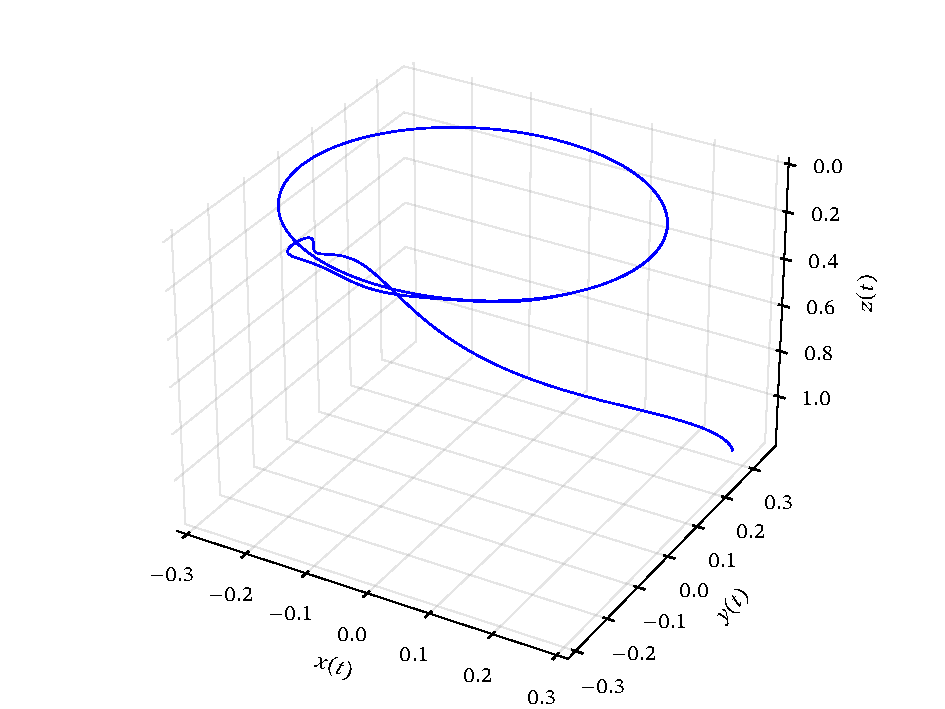
\includegraphics{figures/4results/uav/trajectory.pdf}
    
    \fonte{adapted from \textcite{geronel2023}}
    \label{fig:trajectory}
\end{figure}
Then, it was generated 1000 different trajectories with random noise for each trajectory.
Input and output vector were stored in a MATLAB variable and exported through the \texttt{.mat} extension to be used inside the Python environment using \emph{scipy.io.loadmat} SciPy method.


\section{Algorithm Overview}

The first approach for the ANN is to use the raw data, both for input and output and do the training.
Even though it works, it does not give the proper result, due to the scale for each force and state-space columns.
Therefore, the preprocessing of the data is mandatory to get the best results.
Then, all input and output data were normalized in order to get them all standardized.

The normalization is in L2 form, from the \emph{sklearn.preprocessing.normalize} method, applied in each matrix column.
From the trained ANN, all input data should be normalized and naturally the output also will be normalized.
However, the control forces (output data) can not be normalized to be useful, but there is no ``denormalized'' correspondent matrix to the output data from the ANN.

To solve this problem, a second ANN was created to be able to denormalize the output data.
When preprocessing the data, as the normalization is done, both norms of the input and output data are stored and the second ANN is made from them.
The~\cref{fig:nns_scheme} show how the data and the ANNs are related for the training. 
When the training and the validation is done, the ready-to-use model will perform as shown in the~\cref{fig:full_scheme} scheme.

\begin{figure}[!htb]
    \centering
    \caption[Data and ANN relation]{Data and ANN relation. The training data in the extremes are the ones generated by the white box parametric model.}
    \includesvg[pretex=\footnotesize]{figures/3methodology/nns_scheme.svg}

    \fonte{prepared by the author.}
    \label{fig:nns_scheme}
\end{figure}

\begin{figure}[!htb]
    \centering
    \caption[Model in Production]{Model in production. The scheme shows how the process returns the control forces from the state space.}
    \includesvg[pretex=\footnotesize]{figures/3methodology/full_scheme.svg}

    \fonte{prepared by the author.}
    \label{fig:full_scheme}
\end{figure}

\section{Neural Network Modeling}

The ANN 1 is responsible for, from the normalized state space, to return the normalized control forces.
The problem is considered as a regression problem for both ANNs.
The~\cref{eq:function_training_model_uav} shows the functional form of the ANN 1. Input and output data are all matrices.
%
\begin{subequations}\label{eq:function_training_model_uav}
    \begin{align}
        &f\big(x,y,\ldots,\dot{\theta},\dot{\psi}\big) = \langle U_1, U_2, U_3, U_4 \rangle \\
        &f(\mathbf{X}_s) = \mathbf{T}
    \end{align}
\end{subequations}
%
The  ANN 2 is responsible for, from the raw data, to get the norms from each input and output data of the ANN 1.
The problem is considered as a regression problem.
Input and output data are all vectors.
Both ANNs have similar parameters, being the main difference the input and output layer size.
Characteristics of them are provided in the~\cref{tab:nns_char}.

\begin{table}[!htb]
    \centering
    \footnotesize
    \caption{Parameters of the neural networks and their training}
    \begin{tblr}{
         row{even} = {rosa},
         width=0.8\textwidth,
         colspec={Q[0.5\textwidth,l] Q[0.2\textwidth,r] Q[0.2\textwidth,r]}
    }
    \toprule
    Parameters & ANN 1 & ANN 2 \\
    \midrule
    Input layer neurons   & 12      & 1       \\
    Output layer neurons  & 4       & 1       \\
    Hidden layers neurons & 128     & 128     \\
    Hidden layers         & 8       & 8       \\
    Activation function   & ReLU    & ReLU    \\
    Loss function         & MSE     & MSE     \\
    Optimizer             & Adam    & Adam    \\
    Batch size            & 1       & 1       \\
    Train/test split      & 0.8/0.2 & 0.8/0.2 \\
    Epochs                & 500     & 500     \\
    \bottomrule
    \end{tblr}
    \label{tab:nns_char}

    \fonte{prepared by the author.}
\end{table}


\section{Artificial Neural Networks}

\subsection{Deep Learning}

The concepts of deep learning studied in this section is going to be based on the work of \citet{goodfellow2016} and the documentation of PyTorch\footnote{\url{https://pytorch.org/docs/stable/index.html}} and MATLAB\footnote{\url{https://www.mathworks.com/help/matlab/}}.

There are several definitions of \gls*{ai} \citep{winston1992}, but the  computer scientist \citet{mccarthy2007} defines it as ``the science and engineering of making intelligent machines, especially intelligent computer programs.''.
He also states that ``it is related to the similar task of using computers to understand human intelligence, but AI does not have to confine itself to methods that are biologically observable.''.

The big area of study is the \gls*{ai} and it includes several branches like fuzzy logics, robotics, machine learning and so on. 
The later one, in turn, is another field with also some branches and one of them is the deep learning.
This can be represented in a Venn diagram, as the \cref{fig:venn_dl} shows.
However, all the three terms can be interchangeable in the major context.
%
\begin{figure}[!htb]
    \centering
    \includesvg{figures/3review/nn/venn_dl.svg}
    \caption{Subareas of Artificial Intelligence}
    \label{fig:venn_dl}
\end{figure}

The deep learning history goes back to the 1940s and it had several names over the years. 
It was called by \emph{cybernetics} (1940s--1960s), \emph{connectionism} (1980s--1990s), and from 2006 until now is known as \emph{deep learning}.
The \gls*{dl} models were engineered systems inspired by the biological brain and they were denominated \gls*{ann}.
One of the motivations of the neural  perspective was to understand that the brain provides a proof by example that intelligent behavior is possible and try to reverse engineer the computation principals behind the brain, duplicating its functionality.
Today it goes beyond the neuroscientist perspective and it is more of general principle of learning multiple levels of composition.

\gls*{dl} dwells in the programming sphere. The approach, however, it is not like the traditional programming scripts and models. To automate stuff, there are three main parts: (i) the input data, (ii) the rule (function) and (iii) the output data. In both types there are two of three parts available, but different ones for each other. In the traditional programming, there is the input data and the rule, for the algorithm output the data. In deep learning, there is the input data and the output data, for the algorithm provides the rule. A good analogy is cooking: in the traditional programming context, one has the ingredients and the recipe to make the main course; in the deep learning context, one has the ingredients and the main course to discover the recipe.

\subsection{Neural Networks Models}

Explain how neural networks works.

\begin{figure}[!htb]
    \centering
    \includesvg{figures/3review/nn/nn.svg}
    % \caption[Visual Representation of a Artificial Neural Network]{Visual Representation of a Artificial Neural Network}
\end{figure}

\subsection{Loss Function}

The \emph{loss function}, also called \emph{cost function} or \emph{error function}, is the one used measure the error between the predicted output of an algorithm and the real target output. 
There are several loss functions suitable to different kind of situation. 
For each distributed data there is one that fits better.
The~\cref{fig:mae_chart} represents domain of the loss function.
%
\begin{figure}[!htb]
    \centering
    \includesvg{figures/3review/nn/mae_chart.svg}
    \caption[Loss Function for Linear Regression]{Loss Function for Linear Regression. The loss function take all the distances between the predicted and the target value to verify if the model is in the right path. The lower the distance, the better the model. The \(y\)-axis represents the output data and the \(x\)-axis represents the input data.}
    \label{fig:mae_chart}
\end{figure}

For regression problems, a common loss functions adopted is the \gls*{mse} \citep{bussab2017}. 
%
\begin{equation}
    \mse = \frac{1}{n} \sum_{i=1}^n (y_i - \hat{y}_i)^2
    \label{eq:mse}
\end{equation}
%
where \(n\) is the sample size; \(y_i\) is the predicted output; and \(\hat{y}_i\) is the real target.

\gls*{mse} is a simple method and may lead to poor results if used for the wrong kind of data.

For other data patterns, there are other methods used to get better results for each specific data.

Therefore, the loss function measures how far from the real value the data is. Many kinds of them are available and must be analyzed the most proper one to each case. 
It will depend on not only the data and its pattern, but also the computational processing and the cost attached to it.

\subsubsection*{Cross-Entropy}

From a determined data, there are several classifications that can be extracted from them. 
Their pattern will determine what kind of classification and there are lots of them, like multi-classification, binary classification, regression data, etc.
For multi-classification, the cross-entropy function is a common loss function adopted.

From a distribution \(Q\) relative to a distribution \(P\) over a given set, being both discrete probability distribution, the cross-entropy is defined as
%
\begin{equation}
    H(P,Q) = - \sum_{i=1}^n P(x) \, \log Q(x)
    \label{eq:cross_entropy}
\end{equation}
%
where \(n\) is the size of the sample.

As the~\cref{eq:cross_entropy} is used for multi-classification, the binary cross-entropy, as the name suggest, is used to binary classification. It is defined as
%
\begin{equation}
    H(P,Q) = - \frac{1}{n} \sum_{i=1}^n x \, \log P(x) + (1-x) \, \log \Big(1-Q(x)\Big)
    \label{eq:binary_cross_entropy}
\end{equation}

For classification problems, from the data, the model will try to conclude in what label should the input be classified. 
It is done through probability. 
The cross-entropy measures the ``distance'' between the probability distribution and the true probability, being ideal for this kind of problem.

\subsection{Optimizer}

The optimizer is an algorithm that updates the model in response to the output of the loss function, that is, it aids to minimize the loss function. 
As the loss function minimizes, the model is getting closer to the target values and, hence, closer to the real pattern.

The \emph{gradient descent} is one of the main algorithm \citep{nesterov2004} that optimizes the model and many important ones are based on it, like the \gls*{sgd}. The goal is to get the minimum, as the error (loss) between the predicted and the target data is null. This would mean that the model fits to the pattern of the data.
%
\begin{figure}[!htb]
    \centering
    \includesvg{figures/3review/nn/gradient_descent.svg}
    \caption[Gradient Descent Process]{Gradient Descent Process. In this case, the loss function (yellow curve) can be represented in a two-axes plan. Depending on the data, it is not possible to represent graphically due to its multi dimension. Each point represents the learning step. When the gradient descent reaches the minimum of the loss function, it means that the model may be accurate. Note that the gradient descent can reach a local minimum of the function and not the global minimum necessarily. The \(y\)-axis represents the loss function and the \(x\)-axis represents the weight values.}
\end{figure}

\subsubsection*{Gradient Descent} 

The gradient descent is a powerful algorithm that reduces the loss function, minimizing the error between the predicted value and the target value.

Since the gradient of a function gives the direction of the steepest ascent of a function and it is orthogonal to the surface at a determined point, it seems reasonable that moving in the perpendicular direction gives the maximum increase of the function \citep{stewart2016}.
On the other hand, the negative of the gradient may be used to find the opposite, that is, the steepest descent of the function, or the minimum decrease.
If the steps given to the direction of the negative gradient of the function are small, there is a good chance to get minimum value of the function.
However, if the steps are too long, the chance to pass by the minimum value is high \citep{nielsen2015}.
These steps are called \emph{learning rate} and should be chosen wisely.

This way, let \(\symbf{x}\) be the entry vector with the predicted data and \(L\) the loss function adopted for some deep learning model, and \(\epsilon\) the learning rate, the gradient descent is:
%
\begin{equation}
    \symbf{x}_{t+1} = \symbf{x}_t - \epsilon \nabla L(\symbf{x}_t)
\end{equation}

In determined cases, it is possible to avoid running the iterative algorithm and just go directly to the critical point by solving \(\nabla L(\symbf{x}_t) = 0\) for \(\symbf{x}\).

\subsubsection*{Stochastic Gradient Descent}

As seen, gradient descent is a powerful tool to minimize the loss function, however, for large data, the cost of operation is very high and its use is not feasible. 
The main ideia of \gls*{sgd} is that the gradient is an expectation.
Later, the data is divided in subsets, also called \emph{mini-batch} and then the gradient is performed over them.
The mini-batche size is chosen to be a realatively small numbers of examples.
The data inside each subset may be considered redundant, that is why it uses one single value of the subset to compute the gradient descent.
This way, the process is considerable better for computational resources.

The \gls*{sgd} can be written as:
%
\begin{equation}
    \symbf{x}_{t+1} = \symbf{x}_t - \frac{\epsilon}{m} \sum_{i=1}^m \nabla L(\symbf{x}_t; p^{(i)},q^{(i)})
\end{equation}
%
where \(m\) is the mini-batch size, and \(\nabla L(\symbf{x}; p^{(i)}, q^{(i)})\) is the gradient of the loss function with respect to the parameter vector \(\symbf{x}\) for the \(i^{\text{th}}\) example \((p^{(i)}, q^{(i)})\) in the mini-batch.

Yet, nowadays, with the amount of data, many techniques are still applied in \gls*{sgd} as creating an automatic adaptive learning rates which achieve the optimal rate of convergence \citep{darken1991} and the momentum technique to improve it \citep{sutskever2013}.

\chapter{Literature Review}\label{sec:literature_review}

This chapter deals with the history, the main concepts and some practical cases of \gls*{shm} inside the industry and academic area, besides showing how it may be used in the railway crack detection context.
Next, in the dynamic field, it will be studied the main mechanical concepts to get the necessary understanding to an \gls*{uav} motion as well the basics to know how an \gls*{uav} can be controlled.
Then, it will be shown the mathematics behind the algorithms of deep learning that will be implemented in the \cref{sec:results}. 
Finally, the way how the algorithms are going to be implemented and the tools necessary to achieve the desired \gls*{nn}.
\section{Softwares}

\subsection{PyTorch}
    Reason to why are we using PyTorch \citep{paszke2019}.
    PyTorch is used in Uber\citep{goodman2017}, Tesla\citep{pytorch2019} 
\subsection{Matlab}
    Reasons to why are we using \matlab

\chapter{Literature Review}\label{sec:literature_review}

This chapter deals with the history, the main concepts and some practical cases of \gls*{shm} inside the industry and academic area, besides showing how it may be used in the railway crack detection context.
Next, in the dynamic field, it will be studied the main mechanical concepts to get the necessary understanding to an \gls*{uav} motion as well the basics to know how an \gls*{uav} can be controlled.
Then, it will be shown the mathematics behind the algorithms of deep learning that will be implemented in the \cref{sec:results}. 
Finally, the way how the algorithms are going to be implemented and the tools necessary to achieve the desired \gls*{nn}.

\chapter{Literature Review}\label{sec:literature_review}

This chapter deals with the history, the main concepts and some practical cases of \gls*{shm} inside the industry and academic area, besides showing how it may be used in the railway crack detection context.
Next, in the dynamic field, it will be studied the main mechanical concepts to get the necessary understanding to an \gls*{uav} motion as well the basics to know how an \gls*{uav} can be controlled.
Then, it will be shown the mathematics behind the algorithms of deep learning that will be implemented in the \cref{sec:results}. 
Finally, the way how the algorithms are going to be implemented and the tools necessary to achieve the desired \gls*{nn}.
% ----------------------------

% ============================
% REFERÊNCIAS
% \printbibliography
\bibliographystyle{chicago}
\bibliography{ref}
% ----------------------------

% ============================
% APÊNDICE
\appendix
% \titleformat{\chapter}{\sffamily\centering\bfseries\large}%
% {APPENDIX \thechapter \,--}{1mm}{\large}
% \chapter{Codes}
% ============================
% RELATÓRIO DE PESQUISA
\end{document}